\documentclass[conference]{IEEEtran}
\usepackage[utf8]{inputenc}
\usepackage{graphicx}
\usepackage[table,xcdraw]{xcolor}
\usepackage{subcaption}
\usepackage{biblatex} %Imports biblatex package
\addbibresource{references.bib} %Import the bibliography file
\usepackage{algorithm}
\usepackage[noend]{algpseudocode}
\usepackage{amsmath}
\usepackage{comment}
\usepackage{todonotes}
\usepackage{amssymb, amsmath, amsfonts, amsthm}
\usepackage{mathtools}
\usepackage{bbm}
\usepackage{mathabx} % \vvvert
\usepackage[normalem]{ulem}
\usepackage{tikz}
\usetikzlibrary{shapes.geometric, arrows}



\theoremstyle{remark}
\newtheorem{rmk}{Remark}

%%%%%%%%%
%% Git repositoty https://github.com/nividal/MGARD_bases.git
%%%%%%%%%





\title{Tuning the interpolation basis in a multigrid decomposition for local error control}

\author{\IEEEauthorblockN{Nicolas Vidal}
\IEEEauthorblockA{Oak Ridge National Laboratory}
\and
\IEEEauthorblockN{Qian Gong}
\IEEEauthorblockA{Oak Ridge National Laboratory}
\and
\IEEEauthorblockN{Viktor Reshniak}
\IEEEauthorblockA{Oak Ridge National Laboratory}
\and
\IEEEauthorblockN{Rick Archibald}
\IEEEauthorblockA{Oak Ridge National Laboratory}
\and
\IEEEauthorblockN{Scott Klasky}
\IEEEauthorblockA{Oak Ridge National Laboratory}}

%\author{Nicolas Vidal, Qian Gong, Viktor Reshniak, Rick Archibald, Scott Klasky}
\date{}
\begin{document}

\maketitle



\begin{abstract}
%The compression of scientific data is known a complex problem to be  not only because of the ever-increasing amount of data-involved but also because of the entropy of the floating point representation used in many datasets.
In the compression of scientific data, error-controlled compressor enable to considerably decrease the size of the dataset while maintaining adequate levels of accuracy.
In this paper, we note that multi-level refactoring scheme such as MGARD i) rely on an approximation of the data based on the interpolation of coefficients, ii) estimate the resulting error with global metrics on the dataset.
To improve on these two aspects, we propose a method that aims to divide the original datasets based on their smoothness and refactors each separately with the most relevant interpolation order. We show the relevance of such a method on tailored datasets and the benefits and challenge when applying it to large scientific data.
\end{abstract}

\section{Introduction}
\subsection{Context}
Large scale scientific applications generate an ever-increasing amount of data. %number and ref
The appetite with data in scientific computing is further increased by the development of training models and AI.
In comparison, the bandwidth on existing platforms is limited.
To address these issues, new methods for compression have to be designed and have been a dynamic field of study.
In the case of scientific workflows, there are some additional challenges.
First, datasets produced by these workflows can be hard to compress without loss of accuracy. Indeed compressors rely on the amount of repeating patterns in the data bit representation. However, these repetition can be limited due the prevalent floating-point representation of numbers and the potentially random components of its mantissa~\cite{lakshminarasimhan2013isabela,sayood2017introduction}. %ref

In dataset generated with finite element methods, higher order methods can permit to use less points in order to converge.
The gain in memory at the cost of computational overhead is compensated benefits from the spreading of GPU usage.%\todo[inline]{This looks out of place}

The state-of-the art approach is to use a controlled approximation of the data in order to decrease the entropy before compression~\cite{lindstrom2014fixed,di2016fast,ainsworth2018multilevel}

Another difficulty consists in data-movement from the devices used for generation, usually nodes on a supercomputer, to either local devices used for study or in-situ nodes on the same platform. %ref if needed
In a large and long-lasting simulation, it can be crucial to be able to start processing as soon as possible and potentially before the end of the simulation.
In these circumstances, transferring the most critical portion of the results first provide a valuable gain.
Hierarchical data refactoring is a convenient means for achieving this goal.

These methods permit users to retrieve the adequate amount of data to achieve the required accuracy after re-composition.

Most of this paper uses MGARD: the Multigrid Adaptive Reduction for data ~\cite{ainsworth2018multilevel,ainsworth2019multilevel,ainsworth20quantitative} as an example of multi-level error-bounded compressor but we have the ambition to provide insight for other related tools. %such as?

%provide performance metrics value and refs for MGARD

\subsection{Definition}
A multi-level decomposition scheme provides error control as a theoretical upper-bound of the relative error norm. This relation is conservative, does not depend on the dataset and relies on global norms of the dataset. 
In practice, the actual error bound achieved after decomposition and compression is tied to each specific dataset. In this context, depending on the input, variations on the implementation can yield different results in practice even if they do not impact the theoretical error bound.

In our case, more specifically, we chose to study the impact of order changes in the interpolation method during the decomposition/recomposition steps.
We expect %and show
that using an order fitting the data-resolution can improve the compression ratio and error control of the multi-level decomposition scheme. This is described in Section~\ref{sec:Impact}

In realistic scenario, datasets contains regions of interest that are highly relevant for the scientific study and need high resolution and some less relevant areas, possibly noisy, representing the background or less relevant data points require that much resolution.~(see examples~\cite{ku2016new,ullrich2021tempestextremes,feistauer2015numerical}) %Refs
Therefore, to be usable in such scenario, our method must be able to divide the input into different data blocks according to their characteristics and map an adequate order to each one.

The goal of this paper is to design and present such a solution.
For this purpose, we will address the following problems.
\begin{enumerate}
    \item Given a single block of data, can we achieve better compression ratio by using a specific interpolation order? (Section~\ref{sec:Impact})
    \item Given a data chunk composed of multiple blocks, can we map an order to each data block? (Section~\ref{sec:map})
    \item Given a data chunk, how can we define adequately the different blocks? (\ref{sec:cluster})
\end{enumerate}

\subsection{Contributions}
In this article, we show the relevance of adapting the order of the basis functions used for compression.%\todo[inline]{Maybe should not make an emphasis on higher order necessarily. Variable order? Adaptive order?}
Using different simple synthetic datasets, we highlight an improved compression ratio when the order matches the regularity of dataset.
As it appears unrealistic to use only one basis function order for the entire dataset, we show that we can divide the original data into blocks and compress each separately with a fitting order. 
After validation of these two aspects on examples dataset, we design a complete refactoring scheme including data aggregation for large dataset, subdivision and order mapping, and a decomposition-recomposition scheme. 
Finally, we show the benefits and the challenge of using this method on real-life large scale scientific data.
%Remarks: careful about using "interpolation basis"
% FLOPS Gpu vs CPU costs
% Illustrate the mapping function with mixture + insight on decision

\subsection{Related work}

\paragraph{Lossless compression scheme}
Lossless compression scheme ensures that every bit of the original data remains unchanged in the uncompressed files.
In order to do so, it reduces the redundancy of the information in the original data.
Classical examples include the famous Huffman code, based on the Shannon entropy.
In practice, and especially in scientific data, they achieve limited compression ratios.

\paragraph{Error-bounded compressors}
Error-bounded compressors have been an solution controlling a certain amount of distortion in the compressed data in order to achieve better compression ratio.
Without detailing exhaustively the different compression methods, they have been developed with a certain success in the last years.
Notable examples of such compressors are SZ~\cite{liang2018error} which use dynamic spline interpolation; ZFP, based on orthogonal block transform~\cite{lindstrom2014fixed},
and the hybrid model presented in~\cite{liang2019significantly}.
Isabela\cite{lakshminarasimhan2013isabela} uses BSpline interpolation and apply a preconditioner to noisy data along spatial resolution to provide a fitting model.

They have been shown to provide provide adequate results but are not safe from distortion when the targeted compression ratio is high (~x30)~\cite{liang2019significantly}.

\paragraph{Hierarchical and multigrid techniques}
Using multigrid techniques for compresssion of scientific dataset has mainly been discussed by Ainsworth et al~\cite{ainsworth2018multilevel,ainsworth2019multilevel,ainsworth20quantitative}.
Their proposed compressor, MGARD, will serve as a multi-level decomposition framework for the current article and will be presented in the next section.

\paragraph{Scientific datasets and data smoothness}
%\todo[inline]{Nice paragraph but title should be changed}
 \cite{devore1992image,devore1994classifying} show that natural images have limited smoothness hence is expected to gain limited benefits from using higher orders in wavelet decomposition scheme similar to MGARD.
However, a considerable amount of the scientific data generated and processed in supercomputer comes from high order simulations.
Reference to various dataset are abundant in the literature. %Examples
In the present article, we chose to use SDRBench~\cite{zhao2020sdrbench} for preliminary studies and S3D~\cite{yoo2011direct} as our use case.
%Ref

\section{Overview of MGARD}
\begin{comment}
    \begin{itemize}
    \item Presentation of compression method
    \item Presentation of the basis
    \item Theoretical error bounds for high order
\end{itemize}
\begin{itemize}
    \item Literature review
\end{itemize}
\end{comment}
\subsection{Refactoring pipeline}
MGARD is a multigrid decomposition-based compressor. The decomposition transforms data into coefficients being more suitable to compression.
A $d$-dimensional array $u$ 
% of value $u$ 
as input is interpreted by MGARD as a continuous function having values on a grid $\mathcal{N}_L$ having the same structure as the array.
We can define a series of smaller grids $\mathcal{N}_{L-1},\hdots,\mathcal{N}_0$ downsizing the size by approximately a factor $2^d$ between two consecutive grids. Each grid being a sample of the previous one.
%MGARD decomposition starts from level $L$ on the finest grid $\mathcal{N}_L$ and stops at level $0$ on the coarsest grid $\mathcal{N}_0$.
At each level $l$, the decomposition uses two operations: $L^2$ projection, noted $Q_l$, and multilinear interpolation, noted~$\Pi_l$. % for level l.
The multilevel coefficients on $\mathcal{N}_l \setminus \mathcal{N}_{l-1}$ are the projection $Q_lu$ to the current grid minus its interpolation $\Pi_{l-1}Q_lu$ on the next coarser grid $\mathcal{N}_{l-1}$.
$\Pi_{l-1}Q_lu$ is transformed to $Q_{l-1}u$ using the projection of the coefficients to $\mathcal{N}_{l-1}$.
The procedure is then repeated at the next level.

\begin{comment}
    We can resume the MGARD decomposition procedure as the follows:
\begin{enumerate}
    \item The decomposition starts with $Q_Lu = u$
    \item Compute the piecewise linear interpolant $\Pi_{l-1}Q_lu$ and substract it from $Q_lu$ to get the multilevel coefficients \textsc{$u_mc$} at level $l$. These coefficients encode $(I-\Pi_{l-1})Q_lu$
    \item Project the multilevel coefficients to the coarser level to obtain and add the obtained correction to the interpolant $\Pi_{l-1}Q_lu$ to obtain the $L^2$ projection to the next coarser level, $Q_{l-1}u$.
    \item Repeat the above process until $l=0$.
\end{enumerate}

\end{comment}

\begin{rmk}
For simplicity, in the current article, we chose to discard the projection step for the preliminary studies. It is mostly relevant in the hierarchical representation so the coarser nodes take into account the unrepresented finer levels.
\end{rmk}
    
\paragraph{Error-bounded quantization and Huffman encoding}

The process above transforms the original input into multilevel coefficients $u\_mc$. Allowing lossless recomposition.
To obtain better compression, one could discard either the smallest coefficients or coefficients at the finest level.
A more subtle approach, however, is to quantize the different coefficients, the bin width used in the quantization being directly correlated with the resulting error.
In our experimental pipeline, we use a simple version of the quantization:
\[\sum_{l=0}^L\sum_{x\in \mathcal{N}_l*} |u\_mx[x]-\tilde{u}\_mx[x]| \leq \tau\]

where $\tilde{u}$ is a reduced representation of u after quantization.
MGARD provides guaranties on the error $||u-\tilde{u}||$ for $L^2$ and $L^\infty$. 
%We present the error bounds for the different order basis.
In practice, the error after reconstruction is directly proportional to the bin width used in the quantization.

\begin{comment}
(Figure~\ref{fig:err_vs_binwidth}). 

\begin{figure}[ht!]
    \centering
    \includegraphics[width=0.7\linewidth]{Img/error_vs_binwidth.pdf}
    \caption{Reconstruction error ($L_2$) depending on the bin width used in quantization}
    \label{fig:err_vs_binwidth}
\end{figure}
\end{comment}

    After quantization, the entropy of the dataset decreases and we can apply Huffman encoding. 

    \subsection{Compression}
    In a final step, we compress the resulting data using a standard algorithm in order to study how compressible it is by state-of-the-art algorithms.
    In this study, we chose Zstd~\cite{collet2018zstandard}, a lossless data compression algorithm combining a dictionary-matching stage (LZ77) with a large search window and a fast entropy-coding stage. 
    %It involves Huffman coding and finite-state entropy.

\subsection{Validation}
In order to explore the impact of the interpolation basis on the multi-level decomposition scheme, we implemented our own a framework reproducing MGARD decomposition pipeline with different orders. 
\begin{comment}
    Fig~\ref{fig:sanity} shows that the coefficients obtained by our pipeline decomposition matches those obtained by MGARD for linear interpolant.
We can already notice that for an higher order, coefficients decay faster towards 0. 
\end{comment}
For the experimental evaluation presented in section~\ref{sec:exp}, we will substitute our quantization and compression steps of our pipeline with those of the current release of MGARD. It ensures that these steps fits the state and the art and provide a better comparison of the results.

\begin{comment}
-Figure + reference in the text
-Overlapping with figure 2
-x-axis label
-y-axis label -> explanation on link between magnitude and CR
-more details about dataset

-subfigure b) is too early (comparison between CR of piecewise linear and adaptive)

-> move coefficients magnitude to figure 2

\begin{figure*}
\begin{subfigure}[b]{0.5\linewidth}
    \centering
    \includegraphics[width=\linewidth]{Img/Sanity_coefficients.pdf}
    \caption{Multilevel coefficients obtained by MGARD and different orders of our pipeline on a sample dataset}
\end{subfigure}
\begin{subfigure}[b]{0.4\linewidth}
    \label{fig:sanity}
    \includegraphics[width=\linewidth]{Img/verification_CR.pdf}
    \caption{Compression ratio depending on the source of the coefficients (order 1 - Hurricane dataset)}
    \label{fig:sanity}
\end{subfigure}
\caption{Validation of our pipeline with MGARD}
\end{figure*}
\end{comment}

\section{Impact of interpolation basis order}
\label{sec:Impact}

In this section, we discuss how interpolation basis of different order can have provide different compression ratio for the same error bound, depending on the data refactored. 

\subsection{Motivation}
Arguments to use different orders for decomposition scheme and wavelets transforms have been mentioned in compression literature in various cases.%~\cite{li2023lossy}. %Add 2-3 refs, see wavelets papers
One simple explanation is that different interpolation basis have different properties:
lower orders are easier to compute and require less points so the error propagates less. However they have a low coefficient decay so the amplitude of the error tends to be higher.
Higher orders provide a smoother approach, requiring more points for a more expensive computation. Coefficients decay faster. The error propagates more but with an diminishing amplitude.

In the particular case of scientific data, datasets are often generated using finite element methods.
In this case, an higher order the generation process can permit to use less points in order to converge.
Increasing the order of the finite elements methods is gaining popularity as GPU gain usage, partially compensating the computational overhead.
Intuitively, datasets generated using higher order methods should be approximated more efficiently with higher order interpolation. 

Moreover The accuracy of a decomposition scheme is dependent on the data structure:
	In a smooth dataset (ie continuous with a certain number of continuous derivative),  an  high level interpolation is close to the data, minimizing the coefficients and enabling better compression. Typically such datasets obtained based on analytical functions tend to be smooth.
	In non-continuous data, higher orders represent more computation without this benefit. Typically, natural images are discontinuous datasets.
	Among scientific data, we can find spare datasets, with a high resolve region of interest surrounded by less detailed regions.
    These background regions may contain low values and some noise, having a huge impact of the relative error measurement. Sharp variations between different regions can also make the interpolation imprecise.

    
The intuition would dictate to use high order interpolation for smooth data and lower order interpolation for non-continuous data. For scientific datasets, high-resolve region of interest should be refactored with high order interpolants and the background with low order.
We explore these relations and illustrate with small test cases.

\subsection{Illustration}
As preamble, we illustrate the benefits different interpolation order can represent in a simplistic way:
We try to refactor functions of different orders based on Chebyshev polynomials using different interpolation basis.
This scenario is using only analytical functions and is favorable to high order interpolants
Figure \ref{Fig:Illustration} shows the different compression ratio achieved depending on the interpolation basis used.
As expected, it shows that an order closely fitting the order of the data enables significant compression gains.
Order 0 performs significantly better on the piecewise constant function and poorly in any other scenario. For piecewise linear, order 1 is the best order but order 2 performs decently as well. For functions obtained with higher order polynomials, high order stays better but the relative benefits decrease. 

\begin{figure}[tbh!]
\centering
\includegraphics[width=0.5\textwidth]{Img/error_vs_size_order.pdf}
\caption{Compression ratio obtained for different error depending on the interpolation basis.}
\label{Fig:Illustration}
\end{figure}


\begin{comment}
\begin{figure*}[th!]
\centering
    \begin{subfigure}[b]{0.24\textwidth}
    \centering
        \includegraphics[width=0.9\textwidth]{Img/error_vs_size_order_0.pdf}
        \caption{Piece-wise constant data}
    \end{subfigure}
    \begin{subfigure}[b]{0.24\textwidth}
        \centering
        \includegraphics[width=0.9\textwidth]{Img/error_vs_size_order_1.pdf}
        \caption{Piece-wise linear data}
    \end{subfigure}
    \begin{subfigure}[b]{0.24\textwidth}
        \centering
        \includegraphics[width=0.9\textwidth]{Img/error_vs_size_order_2.pdf}
        \caption{Polynomial data (order 2)}
    \end{subfigure}
    \begin{subfigure}[b]{0.24\textwidth}
        \centering
        \includegraphics[width=0.9\textwidth]{Img/error_vs_size_order_4.pdf}
        \caption{Polynomial data (order 4)}
    \end{subfigure}%
\caption{Compression ratio obtained for different error depending on the interpolation basis.}
\label{Fig:Illustration}
\end{figure*}
\end{comment}


\section{Adaptive solution}

%Presentation
As described in section~\ref{sec:Impact}, scientific data is often obtained from simulation and contains high resolve region of interests and some background consisting of noise and smaller values. These different regions should be refactored differently.
In this section, we present a refactoring solution aiming to split the datasets into blocks containing of similar resolution, mapping an order to each block and refactoring accordingly.

\subsection{Compression pipeline}

\begin{comment}
    
\begin{figure*}
\centering
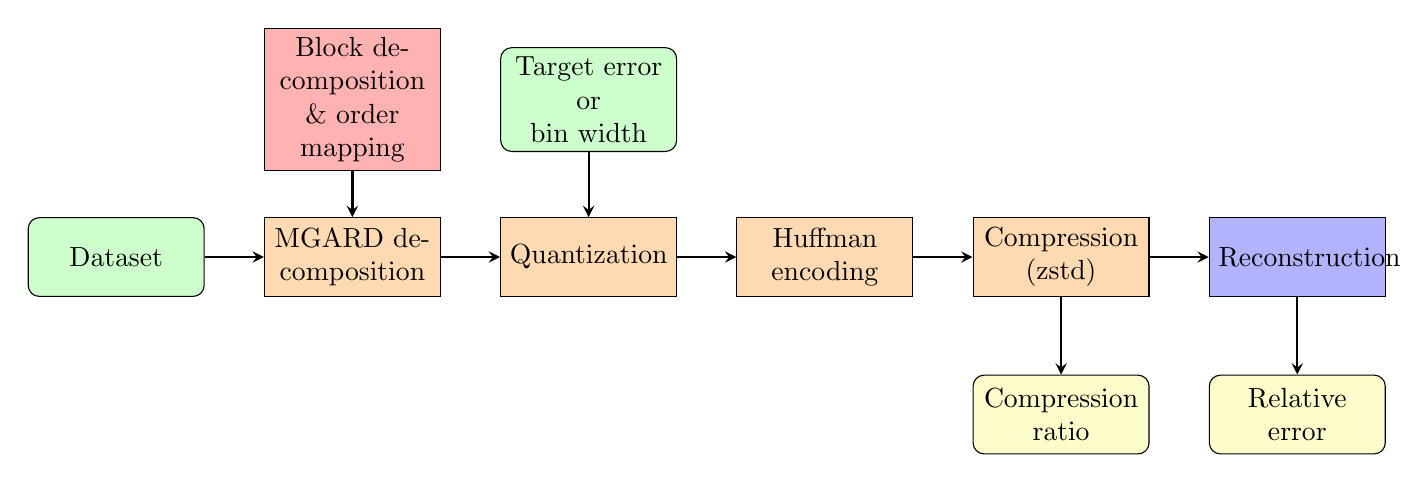
\begin{tikzpicture}[node distance=3cm]
\tikzstyle{input} = [rectangle, rounded corners, minimum width=2cm, minimum height=1cm,text centered, draw=black,text width=2cm,fill=green!20]
\tikzstyle{output} = [rectangle, rounded corners, minimum width=2cm, minimum height=1cm,text centered, draw=black,text width=2cm,fill=yellow!20]
\tikzstyle{comp} = [rectangle, minimum width=2cm, minimum height=1cm,text centered, draw=black,text width=2cm,fill=orange!30]
\tikzstyle{def} = [rectangle, minimum width=2cm, minimum height=1cm,text centered, draw=black,text width=2cm,fill=blue!30]
\tikzstyle{adapt} = [rectangle, minimum width=1cm, minimum height=1cm,text centered, draw=black,text width=2cm,fill=red!30]

\tikzstyle{arrow} = [thick,->,>=stealth]

\node (dt) [input] {Dataset};
\node (mgard) [comp,right of=dt] {MGARD decomposition};
\node (qt) [comp,right of=mgard]{Quantization};
\node (hf) [comp,right of=qt]{Huffman encoding};
\node (zstd) [comp,right of=hf] {Compression (zstd)};
\node (rec) [def,right of=zstd] {Reconstruction};
\node (i1) [adapt,above of=mgard,yshift=-1cm] {Block decomposition \& order mapping};
\node (i2) [input,above of=qt,yshift=-1cm] {Target error\\or\\bin width};
\node (o1) [output,below of=zstd,yshift=1cm] {Compression ratio};
\node (o2) [output,below of=rec,yshift=1cm] {Relative error};

\draw [arrow] (dt) -- (mgard);
\draw [arrow] (mgard) -- (qt);
\draw [arrow] (qt) -- (hf);
\draw [arrow] (hf) -- (zstd);
\draw [arrow] (zstd) -- (rec);

\draw [arrow] (i1) -- (mgard);
\draw [arrow] (i2) -- (qt);
\draw [arrow] (zstd) -- (o1);
\draw [arrow] (rec) -- (o2);


\end{tikzpicture}
\caption{The decomposition pipeline}
\end{figure*}
\end{comment}


In this section, we summarize the compression procedure used by our adaptive method. 
%Chunk
Scientific data is retrieved after generation in form of data \textbf{chunks}. These data chunks are the input of our compression pipeline.
At the start of the compression procedure, each chunk is divided into blocks (for definition of these blocks see section~\ref{sec:blocks}).
Then, an adequate order is mapped to each block (see ~\ref{sec:map}).
At this point, the dataset is divided into blocks of different orders and the compression pipeline is applied each using the adequate order:

The first two steps represent the original MGARD compression pipeline.
\begin{enumerate}
    \item Compute MGARD multilevel decomposition using the selected order decomposition base.
    \item Error-bounded quantization
    \item Huffman encoding of the resulting coefficients
    \item Compression using zstd
\end{enumerate}

Finally, in our different experimental frameworks, we measure the relative errors and compression ratio by comparison with the original data at the end of the whole procedure.

%Validate the benefit of using higher-order basis function  
%Empirically evaluate the achieved compression error vs quantization bin size $\Delta \rightarrow 0$ 



\subsection{Metrics to select the order of basis function}
\label{sec:map}
\paragraph{Interpolation error on the finest grid} 

In the MGARD decomposition pipeline, the multilevel coefficients of the coarse nodes of the grid at level l represent the interpolation error at the given level. We use these multilevel coefficient at finest level to evaluate which order is better.
Lower coefficients for a given order mean that the underlying interpolation base is to be favored.
This can be costly for a large dataset, in this case, a smaller sample can be used. However, the choice of the interpolation order depends on the space-wise distribution of the data and requires a metric computed on the whole region considered.

\begin{comment}
    \begin{figure}
    \centering
    \includegraphics[width=1\linewidth]{Img/placeholder_1stlevel.png}
    \caption{Placeholder -  Illustration of the decomposition scheme. The residual $X^{j+1}$ is used for the mapping function}
    \label{fig:1stlevel}
\end{figure}

\end{comment}

\subsection{Different options for order mapping}
In order to compare two sets of multilevel coefficients, we propose different methods.
\begin{enumerate}
\item L2-norm, the order constructing multilevel coefficient with the smallest L2-norm is used for the decomposition.
  \item Majority voting: For each datapoint, vote for the order providing the smallest multilevel coefficient. After consideration of the whole sample, the order with the most votes is used for the compression.
  \item Entropy-based decision, we compute the entropy of the multilevel coefficients and use the order minimizing its value.
  \end{enumerate}

In the following, we use different rules of thumb to determine the number of bins used to compute the entropy:

\textbf{Freedman-Diaconis' rule:}
\[Nb = \lceil \frac{max(C)-min(C)}{2\times IQR \times n^{-1/3}} \rceil \]
where C is the set of coefficients considered, n the number of coefficients,  Nb is the number of bins and IQR is the difference between the 75-quantile and the 25-quantile.
This rule make no assumption for the coefficients.

\textbf{Scott's rule:}
\[Nb =\lceil \frac{max(C)-min(C)}{3.5 \times s_C \ times n^{-1/3}} \rceil \]
 With the same notations and $s_C$ the standard deviation of the coefficients.
 It assumes normal distribution of the coefficients.

 \textbf{Sturges' rule}
 \[Nb = \lceil 1+log_2(n) \rceil \]
This rules is better for large datasets.


\subsection{Performance}

In this part, we apply our mapping methods on benchmark datasets.
We compress the full dataset using the same order uniformly.
The goal is to show that, given a realistic dataset, we can choose automatically an order improving the ratio.
Figure~\ref{fig:pred2d} compare the performance of the different predictors
For these datasets, an entropy based mapping perform better than other predictors for both Sturge's and Scott's  rules. Majority voting perform worse than the others, indeed it is sensible to variation of large amplitude of the data.

Time comparison of the different order is described in Figure~\ref{fig:time_uniform}. Lower order interpolation are requires less operations than high order ones. We show experimentally that the time gain between order 1 and order 2 is negligible in regards to the full decomposition/recomposition time. However the speed-up for piece-wise constant, which only consist of a very basic operation, is noticeable ($\sim25\%$).


\begin{figure}[h]

    \centering
    \includegraphics[width=\linewidth]{Img/predictors_2d.pdf}
    \caption{Comparison of average normalized compression ratio for different predictors on 2D slices of real datasets}
    \label{fig:pred2d}
%\end{subfigure}
\end{figure}

\begin{figure}[h]

    \centering
    \includegraphics[width=\linewidth]{Img/time_orders.pdf}
    \caption{Decomposition and recomposition time for different interpolation orders}
    \label{fig:time_uniform}
%\end{subfigure}
\end{figure}


\begin{comment}
    
\begin{figure*}
    \begin{subfigure}[b]{0.3\linewidth}
    \includegraphics[width=\linewidth]{Img/uniform/QCLOUDf48.pdf}
    \caption{Caption}
    \label{fig:uQCL}
    \end{subfigure}
        \begin{subfigure}[b]{0.3\linewidth}
    \includegraphics[width=\linewidth]{Img/uniform/RELHUM.pdf}
    \caption{Caption}
    \label{fig:uREL}
    \end{subfigure}
        \begin{subfigure}[b]{0.3\linewidth}
    \includegraphics[width=\linewidth]{Img/uniform/V.pdf}
    \caption{Caption}
    \label{fig:uV}
    \end{subfigure}

\end{figure*}
\end{comment}


\section{Clustering}
\label{sec:cluster}

\subsection{Motivation}
In practice, compression methods are useful for larger datasets.%citation?
In such files, some regions are more resolved or require more precision than others. Additionally, the post-processing can be performed in parallel.
In this context, it could be beneficial, to adapt the order used in data refactoring not to the full dataset but to distinct regions defined upstream.
\begin{figure*}[h]
\begin{subfigure}[b]{0.33\linewidth}
    \centering
    \includegraphics[width=0.90\linewidth]{Img/fun_grid.pdf}
    \caption{\centering Input dataset with tiles of different resolution}
    \label{fig:fun2d}
\end{subfigure}
\begin{subfigure}[b]{0.33\linewidth}
    \centering
    \includegraphics[width=0.90\linewidth]{Img/adaptive_2d.pdf}
    \caption{\centering Compression ratio for the different heuristics}
    \label{fig:cr2d}
\end{subfigure}
\begin{subfigure}[b]{0.33\linewidth}
    \centering
    \includegraphics[width=0.90\linewidth]{Img/time.pdf}
    \caption{\centering Decomposition time for the different policy on the 2D example dataset}
    \label{fig:time}
\end{subfigure}
\caption{2D example on a dataset with region of different resolution}
\label{fig:ex2d}
\end{figure*}


\subsection{Minimal example of composite dataset} 
To demonstrate the relevance of these mapping function, we design a simple example. 
In this section, we focus on the mapping of interpolation orders to different data blocks and not the correct definition of these data blocks.
We construct a input function with the following pipeline.
Defining a set of n intervals $I_{0\leq i \leq n}$ representing a partition of the definition space, and n orders, we define for each interval $I_{i}$ a subfunction of order $o_i$ by interpolating between a set of points (including boundaries points for continuity) with the appropriate Langrange polynomial.
If there is more than 1 dimension, axis are processed one after the other. Example of such a function is shown in Figure~\ref{fig:fun2d}.
This scenario is favorable for large order, as the data generated is very smooth.
The blocks are also too small for Sturge's rule to provide an adequate measure of the entropy. On the opposite, majority voting and norm-based mapping perform better, due to the regularity of the dataset.
In this simple case, based on analytic functions, majority voting seems to perform better as shown in figure~\ref{fig:cr2d}.

\subsection{Time cost of different methods}
Compressing the full dataset with order 0 represent a speedup of around 40\% compared to order 1 and order 2. This gain in lower tiles of lower orders compensate the cost of dividing the datasets and mapping different orders which enables the adaptive method to be performed without overhead as shown in Figure~\ref{fig:time}.

\subsection{Impact of block sizes}
\label{sec:blocks}
With a similar example, we study the impact of the minimum block size imposed to the block decomposition.
Results are shown in Figure~\ref{fig:blocksize}.
Smaller blocks enable a better mapping of the order, resulting to a better compression ratio. In opposite manner, the compression ratio drops when the blocks are too large and include different regions, distorting the mapping function mapping function. With large enough block size, the compression ratio is the same as an uniform compression.
However, the size of the blocks is correlated positively with the time cost of the recomposition scheme.
To summarize, one should pick a block size small enough to enable a good mapping but large enough to avoid excessive recomposition costs. For these datasets, a block size around 100x100 seems adequate.

\subsection{Block definition}

\begin{algorithm}
\caption{Clustering algorithm (Berger-Rigoutsos)}
\label{Alg:Berger}
\begin{algorithmic}
\Require Dataset $B_0$, minimum size $s_{min}$, threshold $\tau$
\State $block\_list \gets [B_0]$;
\State $e_{saved}$ $\gets$ 0 ; saved\_list $\gets$ [$B_0$]
\For {B in block\_list}
\If{$e$(B) $<~\tau$ } 
\State Compute the aggregated votes alongside each axis
\State Find the axis ax with the inflection point p maximizing the gradient
\State Split B at point p orthogonal to axis ax into $B'$ and $B''$
\If {Size($B'$) and size($B''$) $>~s_{min}$}
\State Remove B from block\_list;
\State Add $B'$ and $B''$ to block\_list
\If {$e_{global}$(block\_list) $>$ $e_{saved}$}
\State saved\_list $\gets$ block\_list ; 
\State $e_{saved}$ $\gets$ $e_{global}$(block\_list);
\EndIf
\EndIf
\EndIf
\EndFor
\State block\_list $\gets$  saved\_list
\Return block\_list
\end{algorithmic}
\end{algorithm}


\begin{algorithm}
\caption{Merging function}
\label{Alg:Merge}
\begin{algorithmic}
\Require block\_list
\For {block $B_{i}$ in block\_list}
\For {block $B_{j}$ neighbor of i} \Comment{ie sharing an edge}
\If {order($B_{i}$) = order($B_{j}$)}  
\State add (merge ($B_{i},B_{j}$)) to block\_list
\State remove $B_{i},B_{j}$ from block\_list
\EndIf
\EndFor
\EndFor\\
\Return block\_list
\end{algorithmic}
\end{algorithm}

Define the efficiency of a dataset block B as:
\[e(B) = \underset{i \in orders}{max}( \frac{vote_{i}(B))}{|B|}\] where $vote_{i}(B)$ is the amount of votes for order i in the decomposition of dataset B.
We can extend the definition to a dataset composed of multiple blocks $(B_j)_j$.
\[e_{global}(D) = \underset{j}{min( e(B_i))}\]

Starting from the whole data chunk, the clustering heuristic consists in subdividing the dataset blocks into smaller ones until the global efficiency is greater than a given threshold, typically 80\%.
This is valid as there is no excessive loss in compression ratio when increasing subdivisions. However, past a certain threshold, the time required for additional decomposition/recomposition increases.

\begin{rmk}
    The efficiency of a datablock is defined based on majority voting instead of entropy. It is more convenient for the definition of a absolute threshold as a parameter of the algorithm. It is also more precise for small blocks. Indeed, smaller blocks means that additional subdivision are more costly in terms of decomposition time and impact of the mapping in the resulting relative error. 
\end{rmk}

The full clustering algorithm is described in~\ref{Alg:Berger}, it is a version of the classic Berger-Rigoustos algorithm~\cite{berger1991algorithm}
adapted to our problem.

The core part of this algorithm is to define the best place to split the blocks.
We compute the aggregated votes alongside each axis. After applying a Savitzky–Golay filter to smooth the resulting function, we compute the first and second derivative in order to find a inflection point maximizing the absolute value of the gradient. If multiple coordinates are found on different axis, the one having the largest absolute gradient is picked.
The block is split in two at the given coordinate and orthogonaly at the considered.

In some datasets, the cutting function finds more inflection points than necessary, providing a set of superfluous blocks impacting both the computational cost and the final compression ratio.
Therefore, we chose to save intermediate decomposition in order to pick the best one in the case multiples decomposition do not increase significantly the global efficiency.
Additionnaly, we add a merging step that fuse two adjacent blocks together if they share the same order at the end of the clustering algorithm. Blocks are considered adjacent if they share a full edge. This is done iteratively and results in only rectangular blocks.

\section{Algorithm configuration}
\paragraph{Impact of the efficiency threshold}
%Experiments and discussion
A strict efficiency threshold would, in theory, enable better compression but define an increased number of block, with the risk of reaching the minimal size without significant gain. In contrary, a loose efficiency threshold might not detect regions of different orders.
Preliminary experiments on benchmarks using 1D and 2D datasets show that an threshold of $\sim80\%$ are sufficient.
However, more studies should be performed to properly define a lower bound on efficiency threshold before significant lost in compression ratio and an upper bound before over-resolution leading to no additional gain.


\begin{comment}
The clustering algorithm defines block by subdivising the dataset while a certain threshold of votes is not attained in each block.
The higher the efficiency threshold, the closer the blocks are to have fit the underlying votes but it also means smaller block size.
Experiments show that a threshold of 0.7 or 0.8 is sufficient, in most case, to achieve the best compression ratio.    
\end{comment}



\begin{comment}
\begin{figure}
    \centering
    \includegraphics[width=0.8\linewidth]{Img/BlockQuality.pdf}
\caption{Compression ratio depending on the quality of the order mapping}
\label{fig:quality}
\end{figure}
\end{comment}

\begin{figure}
\begin{subfigure}[b]{0.45\linewidth}
    \centering
    \includegraphics[width=\linewidth]{Img/blocksize_vs_size.pdf}
    \caption{Compression ratio}
    \label{fig:blocksizeCR}
\end{subfigure}
\begin{subfigure}[b]{0.45\linewidth}
    \centering
    \includegraphics[width=\linewidth]{Img/time_recompose.pdf}
    \caption{Recomposition time}
    \label{fig:blocksizetime}
\end{subfigure}
\caption{Impact of block size on compression ratio and recomposition time}
\label{fig:blocksize}
\end{figure}


\subsection{Limitations on real datasets}

Example of a dataset where the mapping function does not provide an good interpolation order.
In some datasets, if the regions have mixed order, the efficiency function based on majority voting can be off:
indeed, an order fitting slightly less points but with a bigger error might be worse than an order providing a smaller error on more points.
In this case, we can weight the amount of votes with the residual norm.

\[ s(o) = \frac{votes(o)}{votes\_total}. \frac{max_{i}||residuals(i)||}{||residuals(o)||}   \]



\paragraph{Cell-based voting groups}

Real datasets contains noise and measurement inaccuracies. These perturbations can result in the interlacing of orders in the voting results making it harder to define the different order regions.
To avoid this issue, we choose to compute aggregate votes on a minimum cell instead of point-wise.
This has also the benefits of reducing the amount of memory required for the clustering, making it easier to deal with larger datasets. Each block can be compressed and reconstructed independently after the blocks definition.

\begin{comment}
\begin{figure*}
\begin{subfigure}[b]{0.33\linewidth}
    \centering
    \includegraphics[width=0.90\linewidth]{Img/Cells/CESM_CLOUD.pdf}
    \caption{\centering Original dataset (CESM Cloud)}
    \label{fig:cell_original}
\end{subfigure}
\begin{subfigure}[b]{0.33\linewidth}
    \centering
    \includegraphics[width=0.90\linewidth]{Img/Cells/cell1.pdf}
    \caption{\centering Pointwise voting}
    \label{fig:cell_1}
\end{subfigure}
\begin{subfigure}[b]{0.33\linewidth}
    \centering
    \includegraphics[width=0.90\linewidth]{Img/Cells/cell40.pdf}
    \caption{\centering Voting on minimum cells}
    \label{fig:cell_40}
\end{subfigure}
\caption{2D example on a dataset with region of different resolution}
\label{fig:ex2d}
\end{figure*}
\end{comment}

\begin{enumerate}
\item Decompose 1st level
\item Divide dataset into cells
\item For each cell, select the order minimizing the L2-norm of the 1st level coefficients
\item Define the different blocks based on the cell decomposition using Berger-Rigoustos algorithm
\item Map the order with a majority of cells to each block
\item Compress each block following the associated order
\end{enumerate}

%Add evidence
\begin{comment}
  \begin{figure}
    \centering
    \includegraphics[width=\linewidth]{Img/Impact_cell.pdf}
    \caption{Impact of cell size on compression ratio - Hurricane dataset}
    \label{fig:Impact_sign_h}
\end{figure}  
\end{comment}

\section{Clustering on real datasets}
\label{sec:exp}
\begin{comment}
\begin{itemize}
\item Synthesized data 
\item Real scientific data 
\item Data which can be partitioned into regions fitting with varied basis functions 
\item Overhead on memory/computation 
\end{itemize}

\begin{enumerate}
    \item Minimal block size
    \item Efficiency threshold
    \item Bin width / Error
\end{enumerate}
\end{comment}

In this section, we compare the performance of our adaptive method on various datasets. 
We used !D linearization and 2D-slices of benchmarks from \url{https://sdrbench.github.io}~\cite{zhao2020sdrbench}.
In order to ensure state-of-the-art compression, blocks and their multilevel coefficients are generated by our framework then compressed the corresponding layer of the MGARD API.
While ensuring the validity of the compression procedure and providing compression ratio more consistent with efficient compressor, it partially hides the memory overhead when the number of blocks increases.
The average compression ratio obtained by the experiments on linearized data are shown in Figure~\ref{fig:adaptive_cr_1d}. Similar results are obtained with 2D slices~\ref{fig:adaptive_cr_2d}. 
The adaptive method (clustering+mapping) show a moderate improvement on compression ratio compared to standard MGARD used as reference.
In the 1D case presented, datasets are decomposed into an average of 5 different segments. However, in the 2D, a majority of the datasets are compressed with uniform orders.

%\paragraph{2D datasets}
% Synthetical "realistic" dataset (x4,5) mix of orders
% realistic datasets (x4,5) -> bigger dataset
% Most important graph (for people who don't read)
% Show it is [almost] always adaptive the best -> 2x is good, 10% don't matter
%s3d include magnitude of velocity as additional variable

\begin{figure}
    \centering
    \includegraphics[width=\linewidth]{Img/adaptive_cr.pdf}
    \caption{Average compression ratio of the adaptive methods (1D)}
    \label{fig:adaptive_cr_1d}
\end{figure}
\begin{figure}
    \centering
    \includegraphics[width=\linewidth]{Img/adaptive_cr.pdf}
    \caption{Average compression ratio of the adaptive methods (2D)}
    \label{fig:adaptive_cr_2d}
\end{figure}

\paragraph{Impact of the voting size}
Increasing the voting group size, improves the clustering algorithm performance, allowing more efficient block definition.
However, providing a large cell size can detrimental for the final compression ratio.
Table~\ref{tab:cell_size} shows that for the benchmarks considered, there is a marginal impact of the voting group size on the compression ratio up to a size of 32x32.

\begin{table}[]
\caption{Impact of the voting group on the compression ratio}
\label{tab:cell_size}
\begin{tabular}{lllll}
\cline{1-4}
\multicolumn{1}{|l|}{Voting group size} & \multicolumn{1}{l|}{CR (1e-3)} & \multicolumn{1}{l|}{CR (1e-4)} & \multicolumn{1}{l|}{CR (1e-5)} &  \\ \cline{1-4}
1 & 9.76 & 5.13 & 3.22 &  \\
\cellcolor[HTML]{EFEFEF}2 & \cellcolor[HTML]{EFEFEF}9.81 & \cellcolor[HTML]{EFEFEF}5.05 & \cellcolor[HTML]{EFEFEF}3.10 &  \\
4 & 9.88 & 5.08 & 3.13 &  \\
\cellcolor[HTML]{EFEFEF}8 & \cellcolor[HTML]{EFEFEF}9.82 & \cellcolor[HTML]{EFEFEF}5.05 & \cellcolor[HTML]{EFEFEF}3.09 &  \\
16 & 9.75 & 5.05 & 3.14 &  \\
\cellcolor[HTML]{EFEFEF}32 & \cellcolor[HTML]{EFEFEF}9.68 & \cellcolor[HTML]{EFEFEF}5.00 & \cellcolor[HTML]{EFEFEF}3.07 & 
\end{tabular}
\end{table}
    


\section{Conclusion}
\begin{comment}
 \begin{enumerate}
    \item optimized strategy for compression
    \item Other compressor
    \item Production code
\end{enumerate}
\begin{enumerate}
    \item Summary of context/contributions
    \item Performance measurement
\end{enumerate}   
\end{comment}
In this paper, we provided insight on why adapting the order of refactoring scheme can benefit scientific datasets using simple experiments.
We have designed a simple and easy to implement method to partition the data and use relevant orders for each block. We discussed the different parameters involved and the various challenge when applying this method to real-life datasets.

Many directions are left to be explored:
In this work, the order is mapped using the order providing the "best" entropy relative to the other. Being able to define absolute threshold instead of comparing different values would help making quantify the improvment of an order compared to the other in terms of compression ratio and would permit to make a decision in the trade-off between time and compression ratio.
The benchmark used for the experiments are relatively small, it would be beneficial to discuss the benefits of the adaptive method and its parameters - including minimum block size, voting group size and signature threshold - on larger and more complex datasets.
Moreover, in this work, we restricted our study to 1D and 2D for the sake of simplicity, applying to datasets with more dimensions could show better performance and also open the option to use different orders alongside different axis.
Finally, after the adequate verification, this adaptive framework should not remain a theoretical object and should be adapted to different decomposition scheme and be included in the production code of some existing compressors.



\printbibliography

\end{document}
